\part{Outils formel}
\pagebreak

\chapter{Logique classique des propositions}
\section{Vocabulaire}

\begin{description}
\item[Déduction] $\models \alpha$ ssi$ \neg \alpha$ est contradictoire
\item[Absurde] $\phi$ est contradictoire ssi $\neg \phi$ est valide
\item[DAG]: Un graphe dirigé acyclique
\item[Taille(Arbre)] = $\{ tout les symboles + connecteurs \}$
\item[Var(Arbre)] = $\{ Toutes les feuilles \}$
\item[Sous formules(Arbres)] = $\{ T + \cup_{i=0}^k SousFormules(Arbre_i) \}$
\item[Interprétation]: $\omega$ de $PROP_{ps}$ est une application de PS dans ${0.1}$
\item[Sémantique]: $\|  \phi \| (\omega)$ d'une formule $\phi$ de $PROP_{ps}$ dans l'interprétation $\omega$ est une élément de ${0.1}$ définit inductive ment par:
\begin{description}
\item[$si \phi \in PS$] alors $\| \phi \| (\omega) = \omega(\phi)$
\item[$si \phi = cX_1 ... X_n$] alors $\| \phi \|(\omega) = C_F(\| x_1 \| (\omega) ... \| x_n \|(\omega))$
\end{description}
\item[$\omega $ satisfait $ \phi$] noté $\omega \models \phi $ ssi $ \| \phi \| (\omega) = 1$
\item[Lorsque $\omega \models \phi$] on dit que $\omega$ est un modèle de $\phi$
\item[on note $\eta(\phi)$] l'ensemble des modèles de $\phi$
\item[$\omega \in PROP_{ps}$ est valide] noté $\models \phi$, ssi toute interprétation $ \omega de PROP_{ps}$ satisfait $ \phi$
\item[$phi \equiv \psi$] sont logiquement équivalents ssi $ phi \models \psi$ et $psi \models \phi$
\end{description}

\section{Propriétés de l'opérateur Models}
\begin{center}
\begin{description}
\item[Réflexivité]: $\phi \models \phi$
\item[Équivalence à gauche]: si $\phi \equiv \theta $ et $ \phi \models \psi $ alors $ \theta \models \psi$
\item[Affaiblissement à droite (transitivité)]: si $ \phi \models \psi $ et $ \psi \models \theta $ alors $ \phi \models \theta$
\item[Coupure]: si $ \cvert{\phi} \wedge \crouge{\psi} \models \cblue{\theta} $ et $ \cvert{\phi} \models \crouge{\psi} $ alors $ \cvert{\phi} \models \cblue{\theta}$
\item[] \scalebox{0.5}{
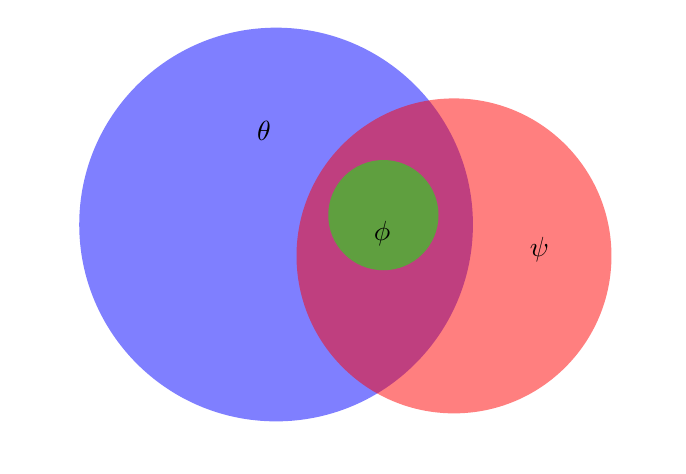
\begin{tikzpicture}
\fill[white](-4,-1) rectangle (4,4);
\fill[opacity=0.5,blue] (0,0) ++(115:2) circle (2.5);
\fill[opacity=0.5,red] (0,0) ++(45:2) circle (2);
\fill[opacity=0.5,green] (0,0) ++(75:2) circle (0.7);
\node[draw=none] at (-1,3) {$\theta$};
\node[draw=none] at (2.5,1.5) {$\psi$};
\node[draw=none] at (0.5,1.7) {$\phi$};
\end{tikzpicture}
}
\item[Ou]: $\cvert{\phi} \vee \crouge{\psi} \models \cblue{\theta} $ ssi $ \cvert{\phi} \models \cblue{\theta} $ et $ \crouge{\psi} \models \cblue{\theta}$
\item[] \scalebox{0.5}{
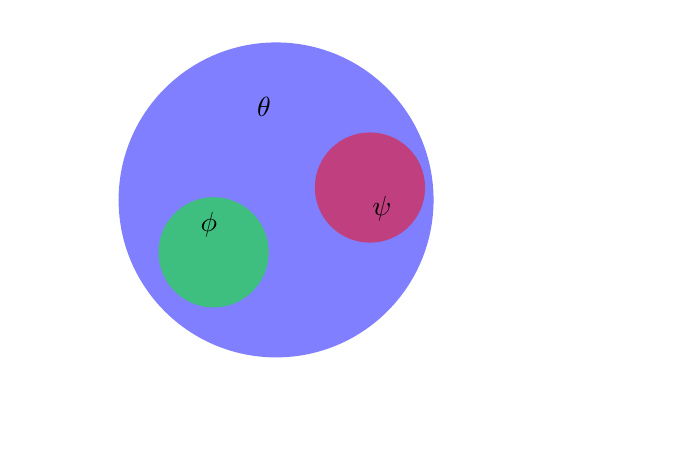
\begin{tikzpicture}
\fill[white](-4,-1) rectangle (4,4);
\fill[opacity=0.5,blue] (0,0) ++(115:2) circle (2);
\fill[opacity=0.5,red] (0,0) ++(80:2) circle (0.7);
\fill[opacity=0.5,green] (0,0) ++(145:2) circle (0.7);
\node[draw=none] at (-1,3) {$\theta$};
\node[draw=none] at (-1.7,1.5) {$\phi$};
\node[draw=none] at (0.5,1.7) {$\psi$};
\end{tikzpicture}
}
\item[Monotonie]: si $\cvert{\phi} \models \cblue{\theta} $ alors $ \cvert{\phi} \wedge \crouge{\psi} \models \cblue{\theta}$
\item[] \scalebox{0.5}{
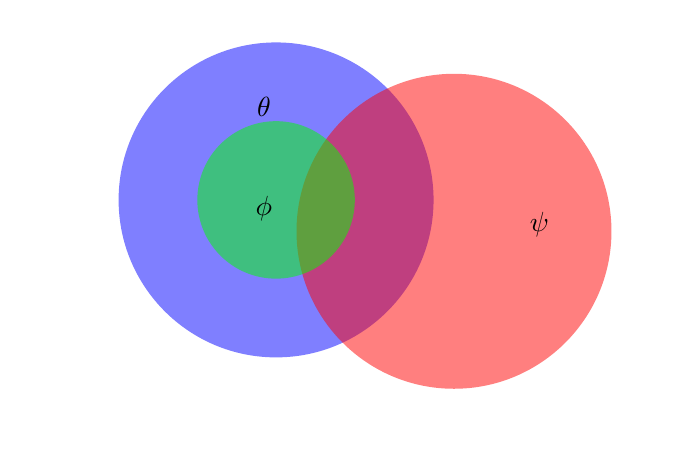
\begin{tikzpicture}
\fill[white](-4,-1) rectangle (4,4);
\fill[opacity=0.5,blue] (0,0) ++(115:2) circle (2);
\fill[opacity=0.5,red] (0,0) ++(45:2) circle (2);
\fill[opacity=0.5,green] (0,0) ++(115:2) circle (1);
\node[draw=none] at (-1,3) {$\theta$};
\node[draw=none] at (2.5,1.5) {$\psi$};
\node[draw=none] at (-1,1.7) {$\phi$};
\end{tikzpicture}}

\end{description}
\end{center}
\pagebreak
\section{Ensemble de connecteurs fonctionnellement complet}
\begin{description}
\item[On dit qu'un ensemble est fonctionnellement complet] si avec que les connecteurs de cette ensemble on peut exprimer toutes les formules d'un monde.
\item[$\{\neg, \wedge\}$] est fonctionnellement complet pour la logique propositionnel classique
\item[] Il en va de même pour $\{\neg, \vee\}, \{vrai, \wedge, \bigoplus\}, \{\neg, \Rightarrow\} ou \{NAND\}$

\begin{description}
\item[Suppression des fils équivalent]: Soit un arbre D ayant comme sous arbre plus d'une fois le nœud $\alpha = (\top X \top)$, $\alpha$ peut être remplacé par $(\top)$ tout en concevant les modèles de D.
\item[fusion des nœuds]: Soit un arbre D ayant comme sous arbre les nœuds $(a B c)$ et $(a` B` c`)$ et $a = a`, b = b`, c = c`$ alors on peut faire relier les deux branches menant vers ces nœuds vers le même sous arbre.
\end{description}
\end{description}

\section{Preuve par induction structurelle sur un ensemble de connecteurs non fonctionnellement complet}

Soit $ \forall P \in \{ \wedge, \vee \}_{ps}$, vérifier P:
\begin{description}
\item[Cas de base $\varphi \in PS$]: $1^\rightarrow (\varphi) = 1$ donc $1^\rightarrow$ constitue un modèle de $\varphi$
\item[Étape inductive]: 
\begin{description}
\item[$\varphi$ s'écrit]: $[\alpha \wedge \beta]$ ou $[\alpha \vee \beta]$
\item[] Avec $\alpha, \beta \in \{ \wedge, \vee \}_{ps}$
\item[] Par hypothèse d'induction, $\alpha et \beta$ vérifient P.
\item[] Il ne reste plus qu'a montrer que $\varphi$ vérifie P.
\item[] $\| \alpha \vee \beta \| (1^\rightarrow)$ = $\vee \models (\|\alpha \|(1^\rightarrow), \| \beta |](1^\rightarrow))$ = $\vee \models (1,1)$ = $1$
\item[] $\| \alpha \wedge \beta \|(1^\rightarrow)$ = $\wedge \models (\| \alpha \| (1^\rightarrow), \|\beta \|(1^\rightarrow))$ = $\wedge \models (1,1)$ = $1$
\item[] donc $x \wedge \neg x$ ne vérifie pas  $P: [| x \wedge \neg x|](1^\rightarrow) = 0$
\end{description}
\end{description}

\section{Décomposition de Shannon}
\begin{description}
\item[On note $\phi [x \leftarrow 0 ) $ ] la formule obtenue en substituant dans $\phi$ la constante faux à toutes les occurrences du symbole propositionnel x.
\item[On note $\phi [x \leftarrow 1 ) $ ] la formule obtenue en substituant dans $\phi$ la constante vrai à toutes les occurrences du symbole propositionnel x.
\end{description}

La décomposition de Shannon de $\phi$ suivant x est la formule:
\begin{description}
\item[] $(\neg x \wedge \phi [x \leftarrow 0]) \vee (x \wedge \phi [x \leftarrow 1])$
\end{description}

\section{Arbre de Shannon, ROBDD}
Étant donnée un ordre strict total $x_1 < x_2 < x_3$ sur $Var(\phi ) = \{x_1, ..... X_n\}$\\
Et une formule $\phi = (\neg x_1 \wedge x_2) \vee ( \neg x2 \wedge x_3)$\\
\begin{tikzpicture}[
  level distance=20mm,
  text depth=.1em,
  text height=.8em,
  level 1/.style={sibling distance=20em},
  level 2/.style={sibling distance=10em},
  level 3/.style={sibling distance=3em},
  every node/.style = {scale=1,
    draw=none, align=center}]]
  \node {$x_1$}
    child { node {$[x_1 \leftarrow \bot]$\\$x_2 \vee (x_2 \wedge x_3)$\\$x_2$} 
      child { node {$[x_2 \leftarrow \bot]$\\$x_3$\\$x_3$}
        child { node {$\bot$ }}
        child { node {$\top$ }}
      }
      child { node {$[x_2 \leftarrow \top]$\\$\top$\\$x_3$}
        child { node {$\top$ }}
        child { node {$\top$ }}
      }
    }
    child { node {$[x_1 \leftarrow \top]$\\$-x_2 \wedge x_3$\\$x_2$}
      child { node {$[x_2 \leftarrow \bot]$\\$x_3$\\$x_3$}
        child { node {$\bot$ }}
        child { node {$\top$ }}
      }
      child { node {$[x_2 \leftarrow \top]$\\$\bot$\\$x_3$}
        child { node {$\bot$ }}
        child { node {$\bot$ }}
      }
    };
\end{tikzpicture}
L'ensemble des modèles de $\phi$ sont toutes les interprétation où la feuille vaut la valeur $T$.

\subsection{Remplacement ou vérifonctionnalité}
\begin{center}
\includegraphics[scale=0.75]{img/of-remplacement.png} \\
\end{center}

$\phi \equiv \phi^{`}$ quelque soit la valeur de x (vrai ou faux).

\subsection{Substitution}
Soit un arbre $D$ ayant comme nœud un sous arbre du type infixe $\alpha = (x \Rightarrow y)$ et un sous arbre de substitution $\beta = (\neg x \Rightarrow \neg y)$\\
$(D^{`} = D_{\alpha \leftarrow \beta} \equiv D$)\\

\section{Notion de impliquant premier }
Les impliquant premier sont des sous formules des formules original tel que ces sous formules soit plus petite que la formule d'origine elle conserve les même modèles:\\
En circuit combinatoire les algo sont appelé  Table de Karnaugh ou Quine-McCluskey.

\subsection{Table de Karnaugh}
Appliquer l'algorithme avec la formule S = $\neg a b \neg c d + a \neg b \neg c \neg d + b \neg d$\\

\begin{center}
\begin{tabular}{l|l|l|l|l}
  \hline
  S & $\neg a \neg b$ & $\neg a b$ & $ab$ & $a \neg b$\\
  \hline
  $\neg c \neg d$ & X & X & X & X \\
  $ \neg c d $ & $ $ & X & X & $ $ \\
  $cd$ & $ $ & X & X & $ $ \\
  $c \neg d$ & X & X & X & X \\
  \hline
\end{tabular}\\
\end{center}

les impliquant premier de S sont $b \neg d$\\

\subsection{Calcule arithmétique}
En logique, les impliquant premier sont calculer que à partir d'une formule en mode CNF transposé en DNF et ensuite détransposé en CNF.

\begin{description}
\item[$\phi$] = $(a \wedge b \wedge c) \vee ( \neg b \wedge c)$
\item[$\phi$] = $(a \vee \neg b) \wedge (a \vee c) \wedge ( b \vee \neg b) \wedge (b \vee c) \wedge (c \vee  \neg b ) \wedge (c \vee c)$
\item[$\phi$] = $(a \vee \neg b) \wedge (a \vee c) \wedge (b \vee c) \wedge (c \vee \neg b) \wedge c$
\item[$\phi$] = $(a \vee \neg b) \wedge c$
\item[$\phi$] = $(a \wedge c) \vee (\neg b \wedge c)$ sont les impliquant premier.
\end{description}

Via une table de Karnaugh:\\
\begin{center}
\begin{tabular}{l|l|l|l|l}
  \hline
  $\phi$ & $\neg a \neg b$ & $\neg a b$ & $ab$ & $a \neg b$\\
  \hline
  $\neg c$ & $ $ & $ $ & $ $ & $ $ \\
  $c$ & X & $ $ & X & X \\
  \hline
\end{tabular}\\
Égal à $(a \wedge c) \vee (\neg b \wedge c)$.
\end{center}

\section{Système de Hilbertien}

g

\section{théorème de finitude}

g

\chapter{Logique classique et prédicat du premier ordre}
\section{Syntaxe via les arbres}
$\phi$ = 
\begin{center}
\includegraphics[scale=0.6]{img/of-occ-1.png} 
\end{center}
\subsection{Occurrences libre}
Une occurrence libre est une variable n'ayant aucun quantificateur associé de son noeud à la racine de l'arbre.\\
par exemple le noeud $y$ ayant un comme contour un losange vert est une occurrence libre, elle sera instancié que lors de l'interprétation de $\phi$.\\
\subsection{Occurrences liée}
Une occurrence liée est une variable ayant un quantificateur associé, comme:
\begin{description}
\item[la variable $x$ entouré d'un rond rouge] est définit via le quantificateur $\forall x$ présent dans ces noeuds parent
\item[la variable $x$ entouré d'un rond violet] est définit par le quantificateur de ces parents $\forall x$
\item[la variable $y$ entouré d'un rond orange] via le quantificateur $\exists y$
\end{description}
A noté que les $x$ entouré d'un rond de couleurs rouge sont diffèrent des $x$ entouré avec un rond orange, donc on peut tout bien renommer les $x$ de couleur orangé en $z$ sans changer le sens de $\phi$.\\
Les occurrences liée se lient sur leur premier père le définissant, comme le $y$ orange qui se définit que sur le $\exists y$ le plus proche de lui.\\
\subsection{Occurrences quantifié}
Les occurrences quantifié sont toutes les variable positionné derrière un quantificateur, celle ci montre comme dans la logique classique, le $\forall$ (où quelque soit) ou $\exists$ (où il existe au moins un).\\
On peut noter que sur la figure ci dessus il y a un $\exists y$ qui n'est pas associé à un $y$ en feuille, on peut s'en débarrasser sans changer le sens de $\phi$.

\subsection{Vocabulaire}
\begin{description}
\item[Formule fermée] est une formule de $FORM_{L}$ qui ne contient aucune variable libre.
\item[Formule instanciée] est une formule qui ne contient aucune occurrence libre ou liée de symbole de variable
\end{description}

\pagebreak
\section{Sémantique}
Soit $t$ un terme de $TERM_L$, la sémantique de $t$ dans l'interprétation de $I$ pour l'assignation $X_i$ noté $[|t|](I)(X_i)$ est l'élément de $D_i$ défini inductivement.

$\phi = $\\
\begin{tikzpicture}[->,>=stealth',shorten >=1pt,auto,node distance=1.5cm,
                    semithick]
  \tikzstyle{every state}=[fill=white,draw=none,text=black]

  \node[state]         (B)                    {$=$};
  \node[state]         (C) [below left of=B]  {$+$};
  \node[state]         (D) [below left of=C]  {$x$};
  \node[state]         (E) [below right of=C] {$2$};
  \node[state]         (F) [below right of=B] {$y$};

  \path (B) edge 			  node {} (C)
        	edge 			  node {} (F)
        (C) edge 			  node {} (D)
        	edge 			  node {} (E);
\end{tikzpicture}

\begin{description}
\item[$=$] $\in \Re$ d'arriter 2
\item[$+$] $\in \Im$ d'arriter 2
\item[$2$] $\in \Im$ d'arriter 0
\item[$X,Y$] $\in X$
\end{description}

Avec une interprétation tel que:
\begin{itemize}
\item[$D_i$] = $\mathbb{N}$
\item[$+_1$] = $\mathbb{N}$ x $\mathbb{N} \rightarrow \mathbb{N}$
\item[$2_i$] = $3$
\end{itemize}

Avec une assignation tel que:
\begin{itemize}
\item[$X_i$]: $X \rightarrow \mathbb{N}$
\item[$ $] $x \rightarrow 5$
\item[$ $] $y \rightarrow 10$
\end{itemize}
\pagebreak
On peut calculer cette sous formule en appliquant chaque terme dans l'interprétation $I$ pour un assignent $X_i$:\\
$\| x + 2 \| (I)(X_i)$ = $+_i ( \| x \| (I)(X_i), \| 2 \| (I) (X_i))$ = $+_i (5,3) = 8$\\
$\| \phi \| (I)(X_i) =$ $ =_i(8,10) = 0 (faux)$\\


$\psi$ = \\
\begin{tikzpicture}[->,>=stealth',shorten >=1pt,auto,node distance=1.5cm,
                    semithick]
  \tikzstyle{every state}=[fill=white,draw=none,text=black]

  \node[state] 		   (A)                    {$\exists x$};
  \node[state]         (B) [below of=A]       {$=$};
  \node[state]         (C) [below left of=B]  {$+$};
  \node[state]         (D) [below left of=C]  {$x$};
  \node[state]         (E) [below right of=C] {$2$};
  \node[state]         (F) [below right of=B] {$y$};

  \path (A) edge              node {} (B)
        (B) edge 			  node {} (C)
        	edge 			  node {} (F)
        (C) edge 			  node {} (D)
        	edge 			  node {} (E);
\end{tikzpicture}

$\| \psi \| (I)(X_i)[x \leftarrow 7]) =$\\
$ =_i ( +_i (\| x\| (I)(X_i [x \leftarrow 7 ]), 3), \| y \| (I)(X_i[x \leftarrow 7])) = $\\
$ =_i ( +_i (7,3), 10) = $\\
$ =_i (10,10) = 1(vrai)$\\

Le quantificateur $\forall$ ou $\exists$ est plus prioritaire que les variables assigné dans $X_i$.\\

Soit $\phi$ la formule $\phi$ ci dessus, la formule interprété avec deux assignations différente:
\begin{description}
\item[$X_i^1$] $x \rightarrow 5, y \rightarrow 10$
\item[$X_i^2$] $x \rightarrow 6, y \rightarrow 10$
\end{description}

L'interprétation de $\phi$ avec $X_i^1$ est équivalent à $\phi$ avec $X_i^2$ car le symbole de quantification $\exists$ est plus prioritaire que les assignations.\\
\pagebreak
\section{Formule polie}
\begin{multicols}{2}
[
Une formule polie est une formule qui pour un nom de variable x, ne porte pas plusieurs significations. Pour se faire il suffit de renommer les variables.\\
La formule de gauche n'est pas sous forme polie, mais celle de droite l'ai:
]
\scalebox{0.5}{
\begin{tikzpicture}[sibling distance=10em,
  every node/.style = {scale=1,
    draw=none, align=center}]]
  \node {$\crouge{\forall x}$}
    child { node {$=>$}
      child { node { $\corange{\exists x}$ }
      	child { node {$\wedge$}
      	  child { node {$P$}
      	    child { node {$\corange{x}$} }
      	    child { node {$y$} }
      	  }
        child { node {$\cblue{\exists y}$}
          child { node {$Q$}
            child { node {$\cblue{y}$} }
          }
        }
      }
    }
    child { node { $\cviolet{\forall y}$ }
      child[missing] {node {}}
      child { node {$P$ }
      	  child { node {$\crouge{x}$} }
      	  child { node {$\cviolet{y}$} }
      	}
      }    
    };
\end{tikzpicture}}
\scalebox{0.5}{
\begin{tikzpicture}[sibling distance=10em,
  every node/.style = {scale=1,
    draw=none, align=center}]]
  \node {$\crouge{\forall x'}$}
    child { node {$=>$}
      child { node { $\corange{\exists x}$ }
      	child { node {$\wedge$}
      	  child { node {$P$}
      	    child { node {$\corange{x}$} }
      	    child { node {$y$} }
      	  }
        child { node {$\cblue{\exists y'}$}
          child { node {$Q$}
            child { node {$\cblue{y'}$} }
          }
        }
      }
    }
    child { node { $\cviolet{\forall y''}$ }
      child[missing] {node {}}
      child { node {$P$ }
         child { node {$\crouge{x'}$} }
         child { node {$\cviolet{y''}$} }
      	}
      }    
    };
\end{tikzpicture}}
\end{multicols}

\section{Équivalences remarquables}
Pour tout $\phi , \psi \in FORM_L$ et $x,y \in X$
\begin{description}
\item[Dualité] $\forall x \phi \equiv \neg \exists x \neg \phi$
\item[] $\forall x ( \phi \wedge \psi ) \equiv (\forall x \phi) \wedge (\forall x \psi)$
\item[] $\exists x ( \phi \vee \psi ) \equiv (\exists x \phi) \vee (\exists x \psi)$
\item[Si $x$ n'est pas libre dans $\psi$ et Q = $\forall$ ou $\exists$ alors]:\\
\begin{description}
\item[] $Qx \phi \equiv \phi$
\item[] $Qx(\phi \wedge \psi) \equiv (Qx \phi) \wedge \psi)$
\item[] $Qx(\phi \vee \psi) \equiv (Qx \phi) \vee \psi)$
\end{description}
\item[] $\forall x \forall y \phi \equiv \forall y \forall x$
\item[] $\exists x \exists y \phi \equiv \exists y \exists x$
\end{description}

\pagebreak
\section{Forme Prénexe}
\begin{multicols}{2}
[
La mise en forme prénexe se fait en transformant la formule en forme polie puis en remontant tout les quantificateurs en haut de l'arbre en fessant attention que lorsqu'on remonte un quantificateur par de la une négation, on applique le duel sur le quantificateur, Et aussi il faut garder l'ordre des quantificateur par rapport à la profondeur de leur sous arbre:\\
(Rappel que $A=>B \equiv \neg A \vee B$):
]
\scalebox{0.9}{
\begin{tikzpicture}[sibling distance=10em,
  every node/.style = {scale=1,
    draw=none, align=center}]]
  \node {$\crouge{\forall x}$}
    child { node {$=>$}
      child { node {$\corange{\exists z}$}
        child { node {$\cblue{\forall a}$ } 
          child { node {$...$}}
        }
      }
      child { node {$\cviolet{\forall y}$}
        child { node {$\wedge$}
          child { node {$x$}}
          child { node {$y$}}
        }
      }
    };
\end{tikzpicture}}
\scalebox{0.9}{
\begin{tikzpicture}[sibling distance=8em,
  every node/.style = {scale=1,
    draw=none, align=center}]]
  \node {$\crouge{\forall  x}$}
    child { node {$\corange{\forall z}$}
 	  child { node {$\cblue{\exists a}$ }
 	    child { node {$\cviolet{\forall y}$}
 	      child { node {$=>$}
 	        child { node {$...$} }
 	        child { node {$\wedge$}
              child { node {$x$}}
              child { node {$y$}}
            }
          }
        }
      }
    };
\end{tikzpicture}
}
\end{multicols}
La partie contenant tout les quantificateurs s'appelle le Prefix et la partie sans quantificateurs s'appelle la Matrice.\\\\
Si dans la formule ci dessus on aurait changé le $=>$ par un $\vee$ (ou autre chose sans signe de négation) les quantificateurs de couleur $\corange{orange}$ et $\blue{bleu}$ ne serait pas "dualisé", mais conserveront l'ordre de leurs profondeur.\\\\
Pareil si on remplace dans la formule le $=>$ par un $\vee$ (ou autre chose sans signe de négation) et on s'intéresse exclusivement au quantificateur $\corange{orange}$ et $\cviolet{violet}$, ($\{\corange{\exists z}, \vee , \cviolet{\forall y}\}$) l'ordre de parcourt des sous arbres n'a aucune importance sur l'arbre final, $(GRD)$ ou $(DRG)$.
\pagebreak

\section{Scalénisation}
\begin{multicols}{2}
[Soit la formule suivante, scaléniser une formule c'est pour tout quantificateurs $\exists y$ dépendant d'un quantificateur $\forall x$, $y$ peut se déduire via une fonction:]
\scalebox{0.9}{
\begin{tikzpicture}[sibling distance=8em,
  every node/.style = {scale=1,
    draw=none, align=center}]]
  \node {$\crouge{\forall  x}$}
    child { node {$\corange{\exists y}$}
 	  child { node {$P$ }
 	    child { node {$\crouge{x}$}}
 	    child { node {$\corange{y}$}}
      }
    };
\end{tikzpicture}
}

\scalebox{0.9}{
\begin{tikzpicture}[sibling distance=8em,
  every node/.style = {scale=1,
    draw=none, align=center}]]
  \node {$\crouge{\forall  x}$}
 	  child { node {$P$ }
 	    child { node {$\crouge{x}$}}
 	    child { node {$func$}
 	      child { node {$\corange{y}$}}
 	    }
    };
\end{tikzpicture}
}
\end{multicols}

\section{Forme propositionnelle}
L'ensemble $SFP(\phi)$ des sous-formules premières de $\phi \in FORM_L$ est défini inductivement par:
\begin{description}
\item[] Si $\phi$ est un atome ou une formule du type $\forall \psi$ ou $\exists \psi$ alors $SFP\phi) = \{\phi\}$
\item[] Si $\phi$ est une formule du type $\neg \psi$ alors $SFP(\phi) = SFP(\psi)$
\item[] Si $\phi$ est une formule du type $\psi \wedge \theta$ ou $\psi \vee \theta$ ou $\psi => \theta$ alors $SFP(\phi) = SFP(\psi) \cup SFP(\theta)$
\item[Si la formule propositionnelle $\phi$ est propositionnellement valide] alors $\phi$ est valide
\end{description}

\begin{multicols}{2}
[]
\scalebox{0.9}{
\begin{tikzpicture}[sibling distance=8em,
  every node/.style = {scale=1,
    draw=none, align=center}]]
  \node {$=>$}
 	  child { node {$\crouge{\forall x}$ }
 	    child { node {$\crouge{P}$}
 	      child { node {$\crouge{x}$}}
 	    }
 	  }
 	  child { node {$\wedge$}
 	    child { node {$\crouge{\forall x}$}
 	      child { node {$\crouge{P}$}
 	        child { node {$\crouge{x}$}}
 	      } 
 	    }
 	    child { node {$\corange{\exists y}$}
 	      child { node {$\corange{Q}$}
 	        child { node {$\corange{y}$}}
 	      } 
 	    }
    };
\end{tikzpicture}
}
$SFP(\phi)$ = $\{$ formules de couleur $\crouge{rouge}$, formules de couleur $\corange{orange}\}\ $,\\ $\phi$ est propositionnellement équivalent à $A => (A \vee B)$ qui est propositionnellement valide donc $\phi$ est valide
\end{multicols}

\chapter{Calculabilité et Machine de Turing}

Soit une machine de turing M un quadruplet M = {K,$\sum$,$\delta$,s)
\begin{description}
\item [K] ensemble fini d'état 
\item [s] $\in$ K état initial
\item [$\sum$] ensemble fini de symboles supposé disjoint de K et de deux symboles:
\begin{description}
\item [$\triangleright$] marque de début
\item [$\sqcup$] séparateur ou fin de ruban
\end{description}
\item [$\delta$]:$(K$ x $\sum)$ x $((K\cup\{yes,no,\uparrow \})$ x $\sum $ x $\{\leftarrow,\rightarrow,-\})$
\begin{description}
\item $\{yes,no\}$ état acceptable
\item $\{\leftarrow,\rightarrow,-\}$ mouvement de la tête de lecture
\end{description}
\end{description}
\pagebreak
\section{Machines de Turing}
Une machine de Turing:
\begin{description}
\item[non déterministe] est une machine qui pour un état $n$ donné peut dériver sur deux état $n+1$ diffèrent (un état est aussi appelé une configuration, une dérivation peu aussi s'appeler une transition).
\item[Déterministe] est une machine qui pour un état $n$ donné n'a qu'une seul possibilité de transition (autrement dit il n'y a que 1 seul $n+1$ unique.
\item[Décideur] est une machine qui pour un mot $x \in L$ termine avec l'indice $yes$ ou $no$.
\item[Accepteur] est une machine qui pour un mot$x \in L$ termine avec l'indice $yes$ ou $\uparrow$ (boucle).
\end{description}

\section{RE, coRE et R}
\begin{description}
\item[Un langage Récursif] (R) pour tout $L \in R$ on peut trouver une Machine de Turing $M$ déterministe qui décide L.\\
$\forall x \in (\sum  \neg \{-\})*$, si $x \in L$ alors $M(x)=yes$ sinon $M(x)=no$.
\item[Un langage récursivement énumérable] (RE) pour tout $L \in RE$ on peut trouver une Machine de Turing $M$ déterministe qui accepte L.\\
$\forall x \in (\sum \neg \{-\})*$, si $x \in L$ alors $M(x)=yes$ sinon $M(x)=\uparrow$.
\item[] (coRE) sont tout les $\{ L \in \rho artie(\sum \neg \{-\})*)$ tel que $L^- \in RE \}$
\end{description}
Remarque: $R \subseteq RE \cap coRE$
\pagebreak
\subsection{Preuve de R est inclue dans RE}
Montrer que $L \in RE$ revient à pour une Machine de Turing Déterministe MT tel que MT accepte L lui associer une output différent.\\
Si on sait qu'il existe un décideur $Mr \in R$, alors construire un accepteur $Ma \in RE$:\\

\begin{tikzpicture}[->,>=stealth',shorten >=1pt,auto,node distance=2.8cm,
                    semithick]
  \tikzstyle{every state}=[fill=white,draw=none,text=black]

  \node[state]         (A)                     {$Ma$};
  \node[state]         (B)  [right of=A]       {$Mr$};
  \node[state]         (YE) [below right of=B] {$yes$};
  \node[state]         (UP) [above right of=B] {$\uparrow$};

  \path (A) edge              node {}      (B)
        (B) edge              node {yes}   (YE)
            edge              node {no}    (UP);
\end{tikzpicture}

\subsection{Preuve de R est inclue dans coRE}
Montrer que $L \in coRE$ revient à pour une Machine de Turing Déterministe MT tel que MT reconnait L lui associer une output différent.\\
Si on sait qu'il existe un reconnait $Mr \in R$, alors construire un accepteur $Ma \in coRE$:\\

\begin{tikzpicture}[->,>=stealth',shorten >=1pt,auto,node distance=2.8cm,
                    semithick]
  \tikzstyle{every state}=[fill=white,draw=none,text=black]

  \node[state]         (A)                     {$Ma$};
  \node[state]         (B)  [right of=A]       {$Mr$};
  \node[state]         (YE) [below right of=B] {$no$};
  \node[state]         (UP) [above right of=B] {$\uparrow$};

  \path (A) edge              node {}      (B)
        (B) edge              node {yes}   (YE)
            edge              node {no}    (UP);
\end{tikzpicture}
\pagebreak
